\documentclass[a4paper,12pt]{article}
\usepackage[utf8]{inputenc}

% bib setup
\usepackage[authoryear]{natbib}
\setcitestyle{numbers,square}
% Bibliography style.
\bibliographystyle{plainnat}

\usepackage{graphicx}
\usepackage{framed}
\usepackage{listings,xcolor}
%\usepackage{inconsolata}

\definecolor{dkgreen}{rgb}{0,.6,0}
\definecolor{dkblue}{rgb}{0,0,.6}
\definecolor{dkyellow}{cmyk}{0,0,.8,.3}

\lstset{
  basicstyle=\ttfamily,
  columns=fullflexible,
  showstringspaces=false,
  commentstyle=\color{gray}\upshape,
  basicstyle=\small,
  numberstyle=\footnotesize,
  numbers=left,
  captionpos=b,
  stepnumber=1,
  numbersep=10pt,
  tabsize=2,
  breaklines=true,
}

\lstset{
  language        = php,
  basicstyle      = \small\ttfamily,
  keywordstyle    = \color{dkblue},
  stringstyle     = \color{red},
  identifierstyle = \color{dkgreen},
  commentstyle    = \color{gray},
  emph            =[1]{php},
  emphstyle       =[1]\color{black},
  emph            =[2]{if,and,or,else},
  emphstyle       =[2]\color{dkyellow}}

\title{Web Engineering: Miniproject}
\author{Jesper Riemer Andersen\\Nicklas Andersen\\Simon Reedtz Olesen}

\begin{document}
\maketitle

\section{Block 1: Introduction}
We have simple 3-tier architecture which allows us to communicate with the server and extract data from our database. This protects the database from unwanted queries from the client.

\begin{center}
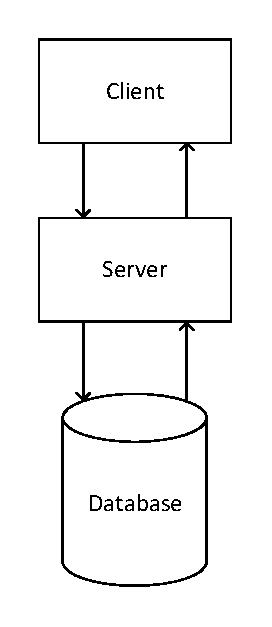
\includegraphics[scale=0.8]{3-tier.pdf}
\end{center}

\begin{enumerate}
\item The client opens his web browser and sends a HTTP request to the server.
\item The server runs the PHP script which queries data from the database.
\item The database returns the result according to the query.
\item Then the server returns the HTTP response to the client.
\item The response is then output as HTML.
\end{enumerate}

\begin{lstlisting}[language=php,label=lst:aspectratio] 
<?php
$connection = mysql_connect("localhost", "root", "");
mysql_select_db("webengi", $connection);

$query = mysql_query("SELECT testtext FROM hello", $connection);

while ($row = mysql_fetch_assoc($query)) {
    echo $row['testtext']."</br>";
}
?>
\end{lstlisting}

This code shows the steps explained above. We chose to run the server on localhost using WampServer, which also comes bundled with a MySQL database.

We start by connecting to the localhost with the username \textit{root} and empty password. Then we select the database called \textit{webengi}, and then query the database. For each row that is returned by the query, we echo the content of the column called \textit{testtext}.

\section{Block 2: Data I: XML etc.}

We found an XML document containing a small set of computers for sale on eBay, which we will display a subset of. We will be using the following:
\begin{itemize}
\item An XML file containing data on computers for sale.
\item An XSL file with our XSL transformations (XSLT).
\item A HTML file which contains only a little javascript to load the other files and display the result.
\end{itemize}

\begin{lstlisting}[language=xslt,label=lst:xslt] 
<?xml version="1.0" encoding="ISO-8859-1"?>
<xsl:stylesheet version="1.0" xmlns:xsl="http://www.w3.org/1999/XSL/Transform">

<xsl:template match="/">
  <h2>Computers for sale on eBay</h2>
    <table border="1">
      <tr bgcolor="#9acd32">
        <th>Current bid</th>
        <th>Memory</th>
        <th>Hard drive</th>
        <th>CPU</th>
      </tr>
      <xsl:for-each select="root/listing">
      <tr>
        <td><xsl:value-of select="auction_info/current_bid"/></td>
        <td><xsl:value-of select="item_info/memory"/></td>
        <td><xsl:value-of select="item_info/hard_drive"/></td>
        <td><xsl:value-of select="item_info/cpu"/></td>
      </tr>
      </xsl:for-each>
    </table>
</xsl:template>
</xsl:stylesheet>
\end{lstlisting}

This is the XSL file with our transformation. The following box is copied from w3schools.com \citep{w3xslt}.

\begin{framed}
Since an XSL style sheet is an XML document, it always begins with the XML declaration: \lstinline$<?xml version="1.0" encoding="ISO-8859-1"?>$.

The next element, \lstinline$<xsl:stylesheet>$, defines that this document is an XSLT style sheet document (along with the version number and XSLT namespace attributes).

The \lstinline$<xsl:template>$ element defines a template. The \lstinline$match="/"$ attribute associates the template with the root of the XML source document.

The content inside the \lstinline$<xsl:template>$ element defines some HTML to write to the output.
\end{framed}

\subsection{XML vs XSLT}

XQuery and XSLT are two languages used for quering XML. We have chosen to experience a bit with both  to find out how they worked.

We spent a lot of time trying to make XQuery work with PHP Zorba. Zorba is a sort of virtual machine for query processing, however we could not make it work with the newest version of PHP for some reason, so we ended up using an Eclipse plugin called  "Sausalito Tools" for the Xquery, allowing us to read an XML document and extract information but we did not connect it to our database. 

It allowed us to get a general understanding of XQuery and XPath and how to extract information from an XML file using these queries. 

XSLT is primarily conceived as a stylesheet language used to render XML on screen where as XQuery is conceived as a database query language and in our case our main focus is to query an XML file in our database and not styling our website. 

XSLT is stronger when it comes to making small changes to a document, because it can make use of a coding pattern that involves a template that copies all nodes unchanged, modified by specific templates that modify selected nodes.

XQuery does not support dynamic binding or polymorphism, but this ability is more noticeable when writing large applications, which we do not expect to be doing. 

\subsection{Block 4: Architecture}

For the architecture we used a Model-View-Controller.

This allows us to divide our application into three kinds of components;

\begin{itemize}
\item A model is a representation of some data in a domain. It is an object containing all data and behaviour, other than that used for the UI. 
\item The view represents the display of the model in the UI. The view is only about displaying the information, any changes that might be made to the data is handled by the controller. 
\item The controller takes user input and manipulates the model and the view is updated appropriately. 
\end{itemize}

\subsubsection*{Model}

\subsubsection*{View}
We chose to use the Template View because it is easy to implement and for our assignment we only needed to display a static HTML page because our data was also static.

If we had dynamic data, it might have been more appealing to use a Transform View where we would have used the data as input and "transformed" it into HTML, thus giving us a more dynamic HTML view for different sorts of data.

If we had had more than one web page, a two step view could have been appealing to use. It allows you to have a consistent look and organization across your website. 

Due to the simplicity of our dataset, a template view was more than sufficient with its easy implementation it was very appealing for us. 

\subsubsection*{Controller}


\subsubsection*{Advantages and disadvantages of MVC}

\paragraph{Advantages}
\begin{itemize}
\item It is possible to substitute and re-use views and controllers for the same model.
\item Many views for the same model 
\item Clear separation between presentation logic and business logic
\item Easy to maintain code for future improvements
\item All views are synchronized and reflect the current state of the model 
\item It is easy to test the core of the application
\end{itemize}

\paragraph{Disadvantages}
\begin{itemize}
\item Increased complexity because an application can use other patterns at the same time as MVC (for example in an active model using an Observer pattern)
\item Changes to the model require changes in the view and might require changes to the controller as well.
\item It is very difficult to have a strict separation between view and controller. 
\end{itemize}
\bibliography{bibliografi}
\end{document}